\chapter{Experimentelle Untersuchungen im Windkanal}
\label{s:versuche}
%%%%%%%%%%%%%%%%%%%%%%%%Modellbeschreibung Tim%%%%%%%%%%%%%%%%%%%%%%%%%%%%%
\section{Das Versuchsmodell (TG)}
\label{sec:Modell}
Die Versuche werden am gleichen Modell duchgef"uhrt, welches im Zuge der Arbeit von Bilges \cite{Bilges.2018} verwendet wurde. Die Form entstammt der Arbeit von Oswald \cite{Oswald.2017}. Eine Skizze des Modells ist in \abb{fig:SkizzeModell} zu sehen.

\begin{figure}[h]
	\centering
	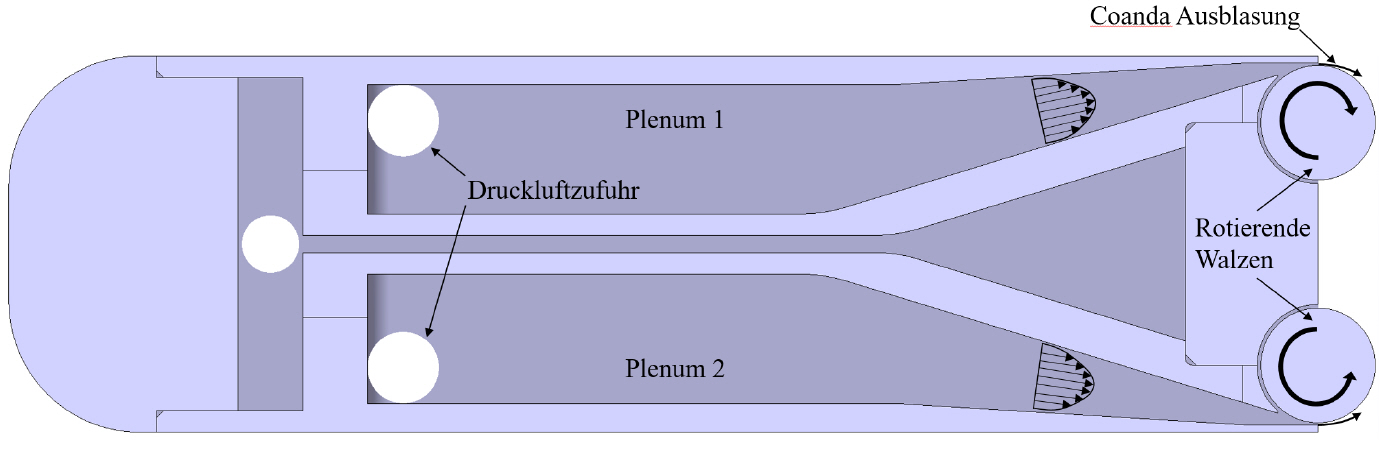
\includegraphics[width=0.9\textwidth]{SkizzeModell.jpg}
	\caption{Skizze des Versuchsmodells \citep{Bilges.2018}}
	\label{fig:SkizzeModell}
\end{figure}

Im Inneren teilt sich der Stumpfk"orper in zwei Kammern auf, welche mit Plenum 1 und Plenum 2 an der Ober- respektive Unterseite des K"orpers bezeichnet sind. "Uber die eingezeichneten "Offnungen im vorderen Teil werden die beiden Plenen "uber 4 Druckluftschl"auche mit bis zu 8 bar Druckluft versorgt, wobei diese in den Hinterteil des K"orpers str"omt. Hier findet durch den eingezeichneten Spalt eine Coanda-Ausblasung "uber die entgegengesetzt rotierenden Walzen aus Kapitel \ref{s:rotierendeWalzen} statt.

Zur Bestimmung der Oberfl"achendr"ucke sind entlang der K"orperkontur mittig an der Ober- und Unterseite 32 Druckluftbohrungen platziert worden. Die Position der Bohrungen sowie die folgend beschriebene Geometrie des K"orpers ist in \abb{fig:ModellGeometrie} ersichtlich. Das Modell kann als D-Stumpfk"orper klassifiziert werden und hat folgende Abmessungen: 
\begin{center}
H"ohe: h = 53,4 mm\\
Breite: b = 390 mm\\
L"ange: l = 190,6 mm\\ 
\end{center}
Dabei ist die Breite des Modells so gew"ahlt, dass dessen Seiten inklusive Fl"achendichtungen b"undig an der Windkanalwand abschlie\ss{}en. 

\begin{figure}[h]
	\centering
	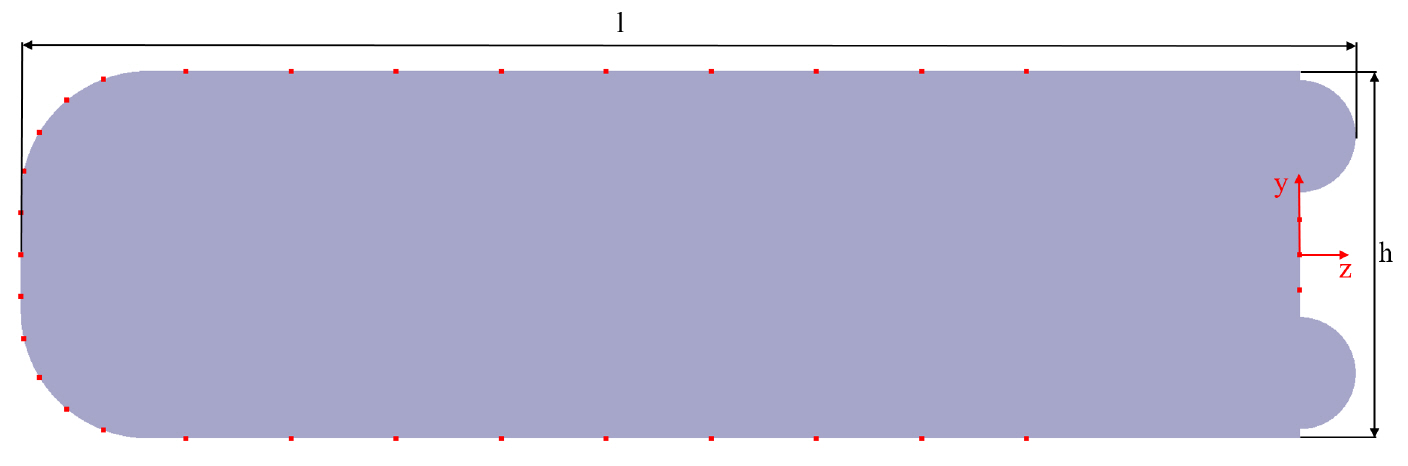
\includegraphics[width=0.75\textwidth]{ModellGeometrie.jpg}
	\caption{Geometrie des D-Stumpfk"orpers mit eingezeichneten Druckbohrungen \citep{Bilges.2018}}
	\label{fig:ModellGeometrie}
\end{figure}

Die oben erw"ahnten Druckmessbohrungen sind in \abb{fig:DModell1} erkennbar. Deren Messschl"auche werden vorne an den Seiten des Modells herausgef"uhrt. Die Aluminiumholme rechts und links dienen zur Aufh"angung und genauen Justierung des Modells innerhalb des Windkanals. Die beidseitig sichtbaren Messinganschl"usse sind die bereits erw"ahnten Anschl"usse f"ur die Druckluft.
Wie bereits in Abschnitt \ref{sec:Vorderkante} erl"autert wurde, erzeugt die Vorderkante eine laminare Abl"oseblase, wie es in \abb{fig:LamBlase} dargestellt ist. Um Str"omungsabl"osungen zu vermeiden, wird daher an der Vorderkante des Modells an der Ober- und Unterseite ein Zackenband befestigt. Dieses Band, welches vor der Abl"osezone befestigt wird, dient als Wirbelgenerator und sorgt daf"ur, dass die laminare Str"omung zwangsweise in turbulente Str"omung umgewandelt wird. Auf H"ohe der Abl"oseblase sorgt die Turbulenz zu einem Engergietransport quer zur Anstr"omung, was dazu f"uhrt, dass die Abl"oseblase geschlossen wird und die Str"omung fr"uher wieder anlegt.

\begin{figure}[h]
	\centering
	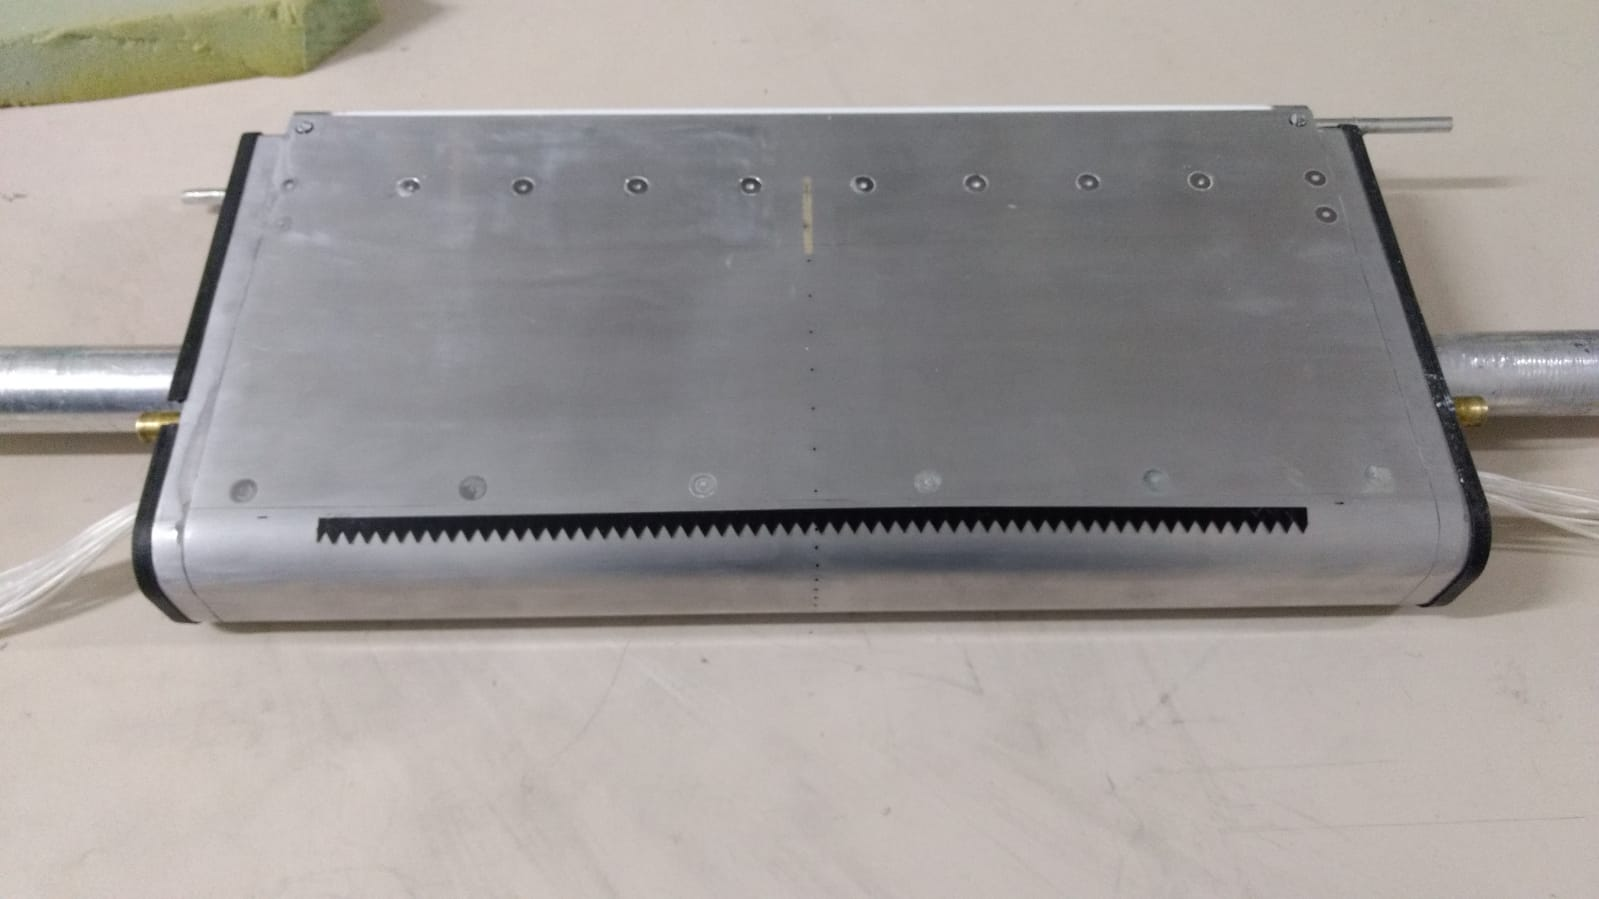
\includegraphics[width=0.55\textwidth]{DModell1.jpg}
	\caption{Vorderansicht des Versuchsmodells mit Zackenband an Ober- und Unterseite.}
	\label{fig:DModell1}
\end{figure}
Wie in \abb{fig:DModell2} ersichtlich ist, sind an der R"uckseite des Stumpfk"orpers an Ober- und Unterseite des Modells jeweils 10 Schrauben montiert. Diese dienen der Einstellung des Ausblasespaltes. Das genaue Verfahren zur Einstellung des Spaltes wird in Abschnitt \ref{sec:Versuchsvorbereitung} erl"autert.


%\begin{figure}[h]
%	\centering
%	\begin{subfigure}[c]{0.49\textwidth}		
%		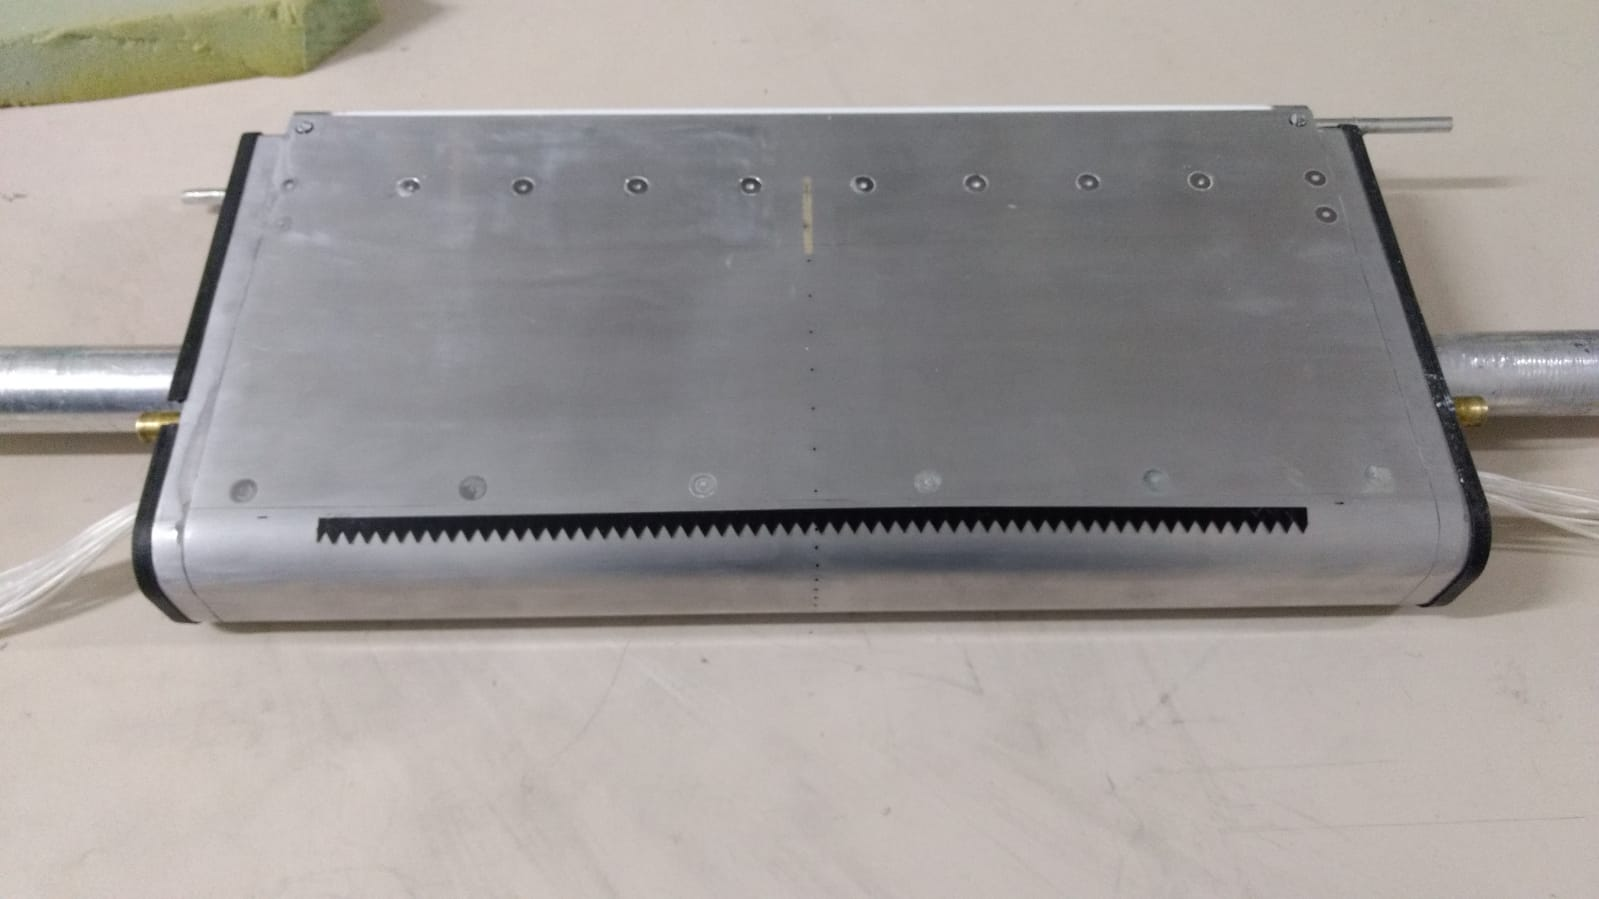
\includegraphics[width=1\textwidth]{DModell1.jpg}
%		\subcaption{Vorderansicht mit Zackenband an Ober- und Unterseite.}
%		\label{fig:DModell1}
%	\end{subfigure}
%	\begin{subfigure}[c]{0.49\textwidth}
%		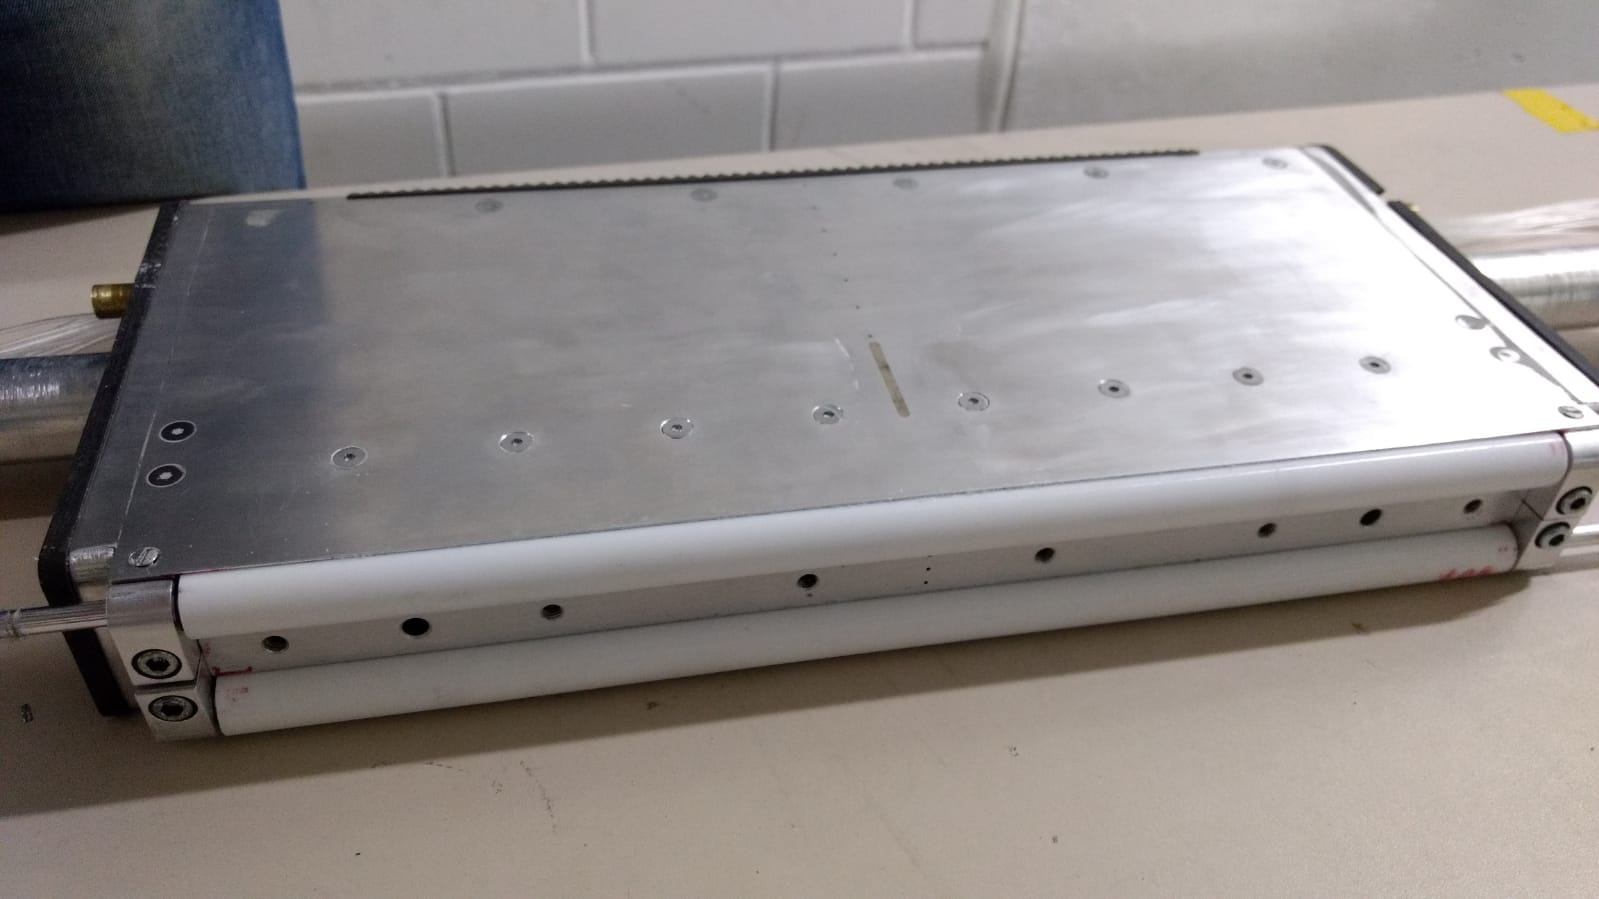
\includegraphics[width=1\textwidth]{DModell2.jpg}
%		\subcaption{R"uckansicht mit eingebauten Tefolnwalzen.}
%		\label{fig:DModell2}
%	\end{subfigure}
%	\caption{Ansicht des Versuchsmodells}
%	\label{fig:DModell}
%\end{figure}


\begin{figure}[h]
	\centering
	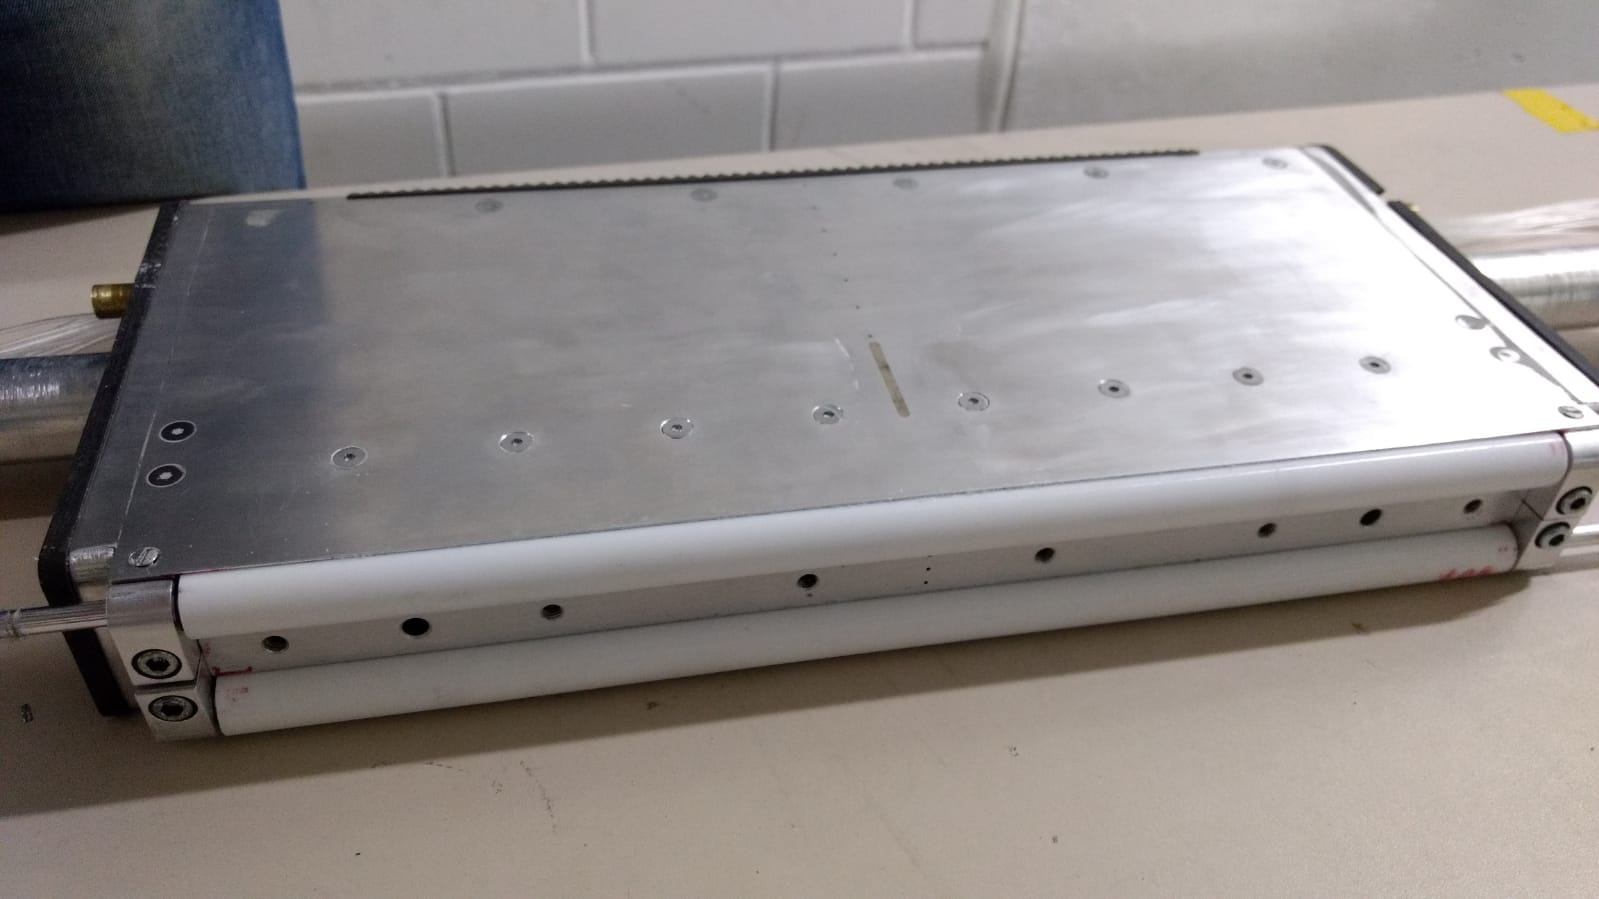
\includegraphics[width=0.55\textwidth]{DModell2.jpg}
	\caption{R"uckansicht des Versuchsmodells mit eingebauten Tefolnwalzen.}
	\label{fig:DModell2}
\end{figure}

\clearpage
%%%%%%%%%%%%%%%%%%%%%%%%ENDE Modellbeschreibung Tim%%%%%%%%%%%%%%%%%%%%%%%%%%%%%



%%%%%%%%%%%%%%%%%%%%%%Kebria%%%%%%%%%%%%%%%%%%%%%%%%%%%%%%%%%%%%%

\section{Windkanalbeschreibung (KK)}
F"ur die experimentellen Untersuchungen steht der LNB (Leiser Niedergeschwindigkeitskanal Braunschweig) vom Institut f"ur Str"omungsmechanik der technischen  Universit"at Braunschweig zur Verf"ugung.\\
Dieser ist an beiden Enden offen und wird durch die Umgebungsluft im Raum versorgt, was als Eiffel-Bauart bezeichnet wird. (\abb{fig:windkanal}).
Durch eine besondere Art der Polsterung bzw. Schalld"ampfer und einen
ger"auscharmen Elektroantrieb, ist dieser Windkanal so f"ur einen m"oglichst leisen Betrieb konstruiert worden.
\begin{figure}[h]
	\centering
	\begin{subfigure}[c]{0.5\textwidth}		
		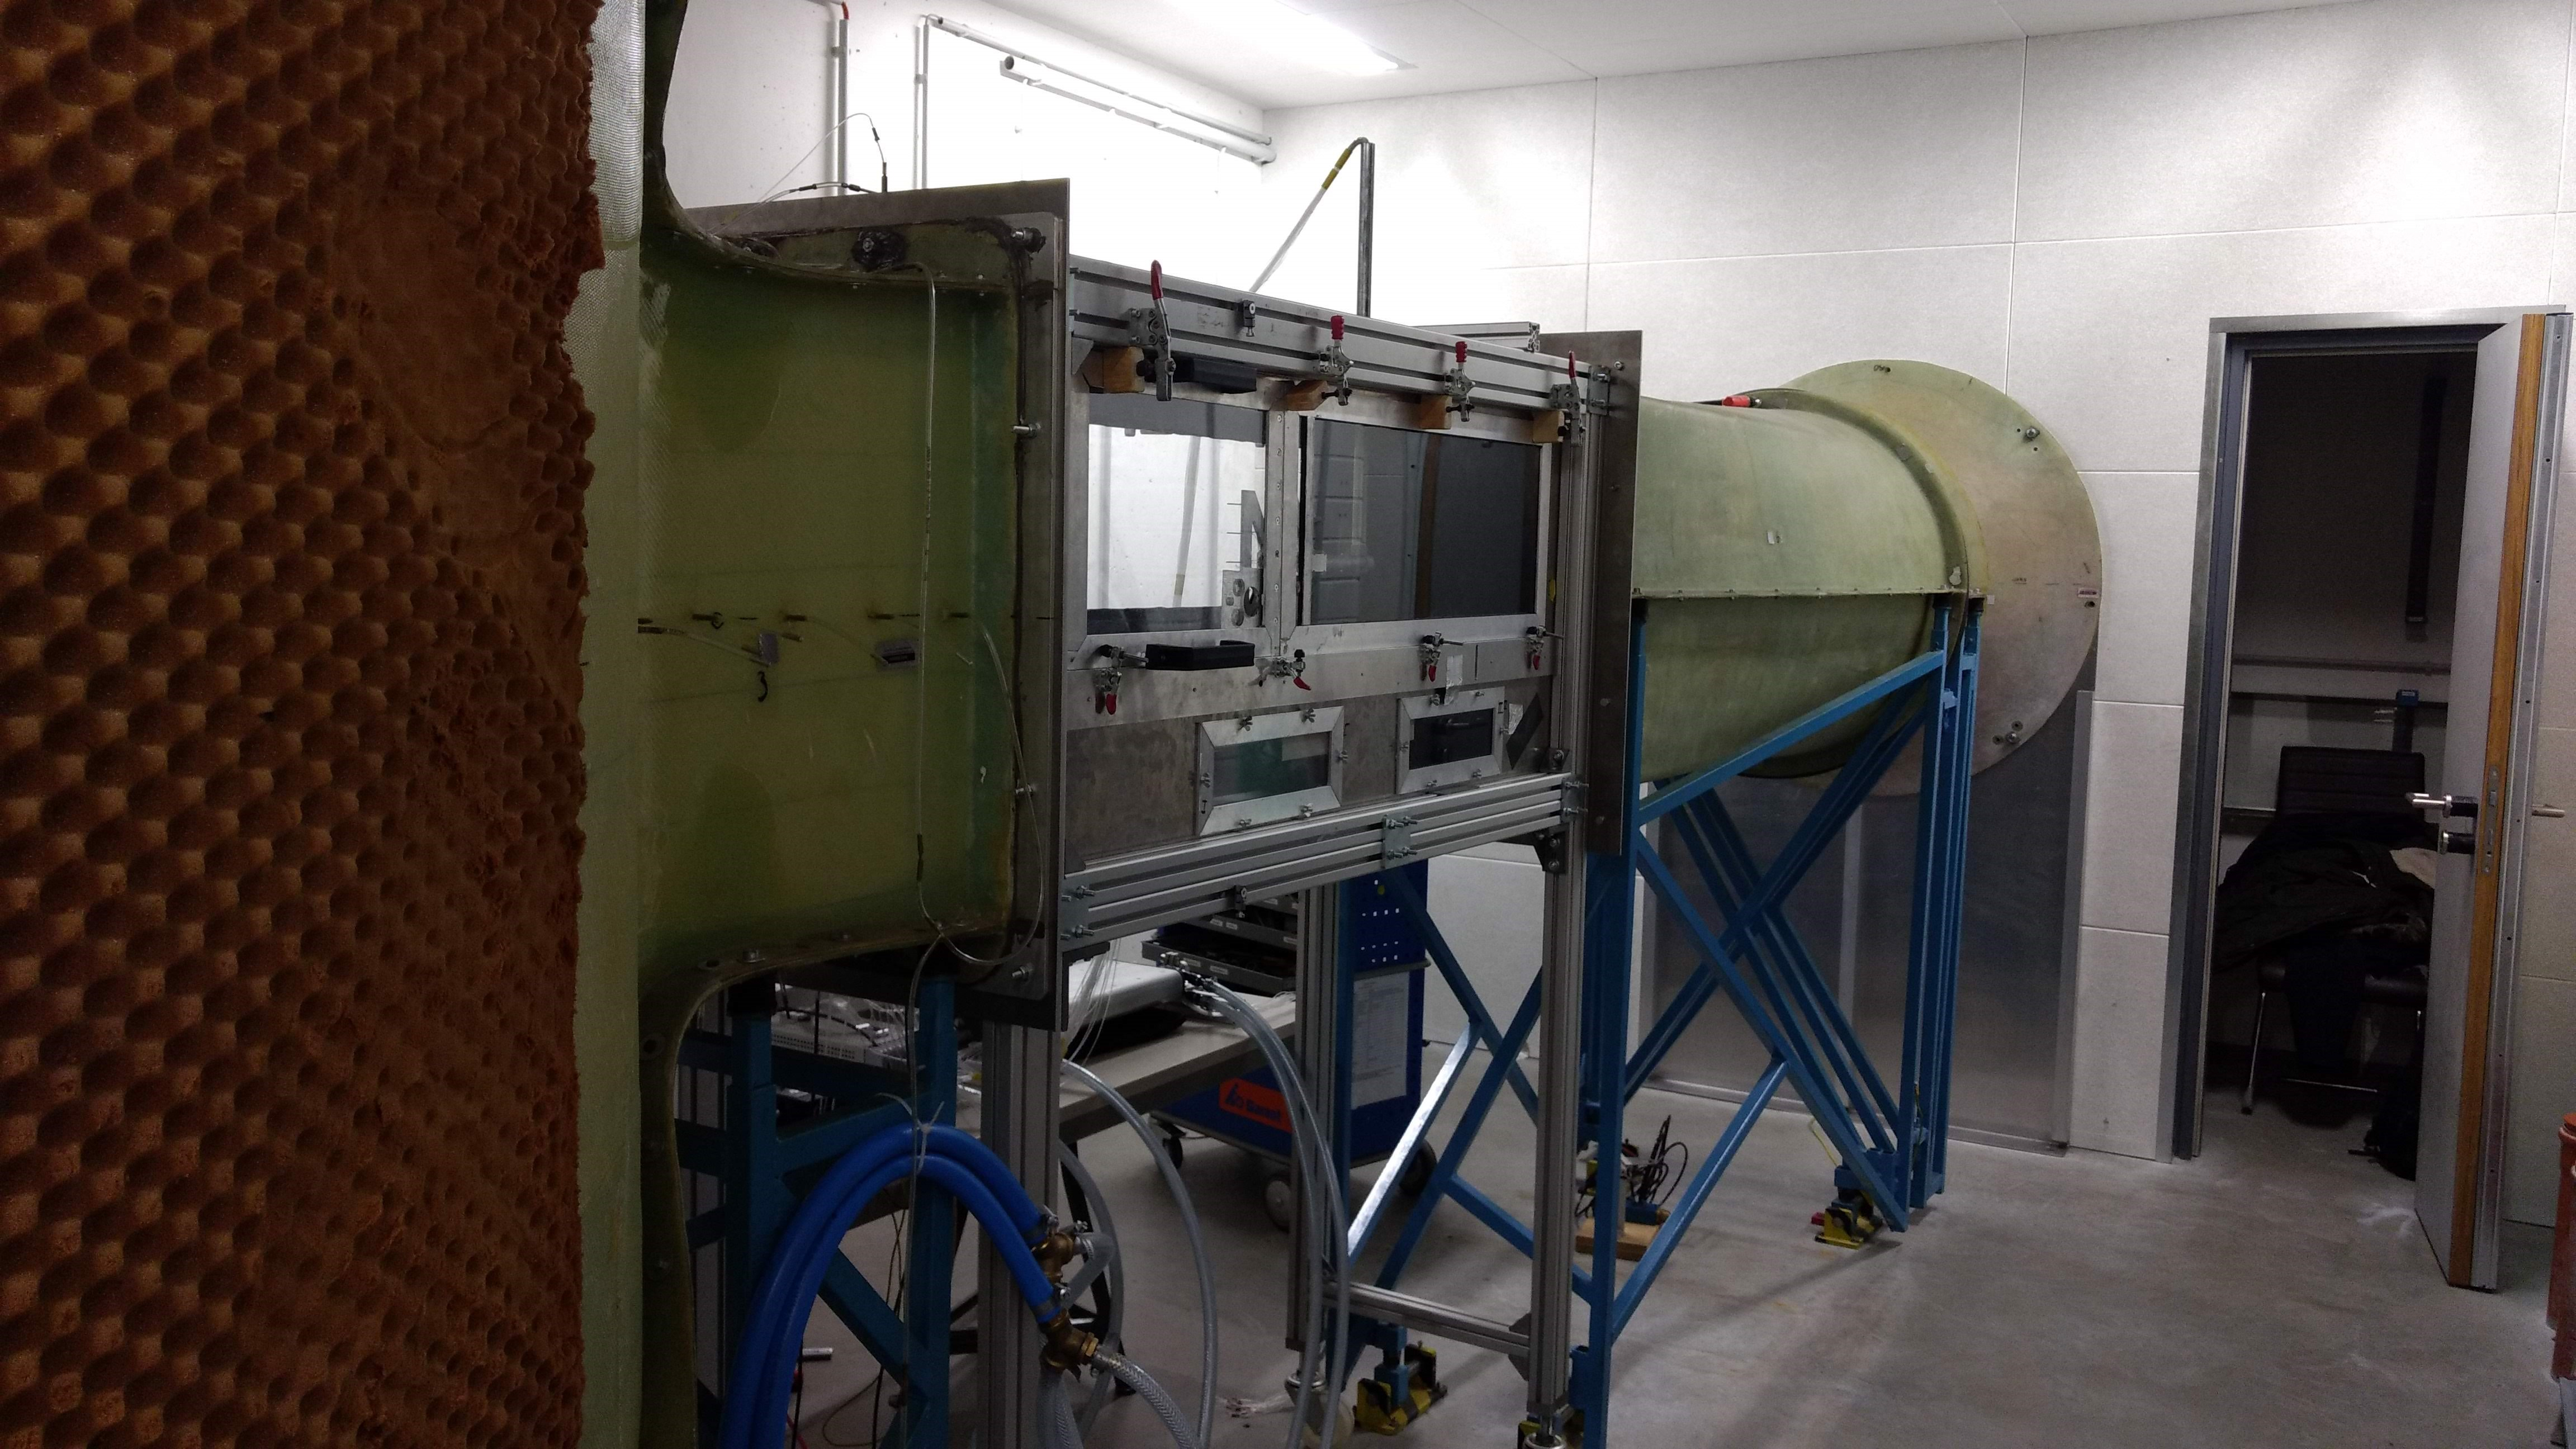
\includegraphics[width=1\textwidth]{windkanal1.jpg}
	\end{subfigure}
	\begin{subfigure}[c]{0.5\textwidth}
		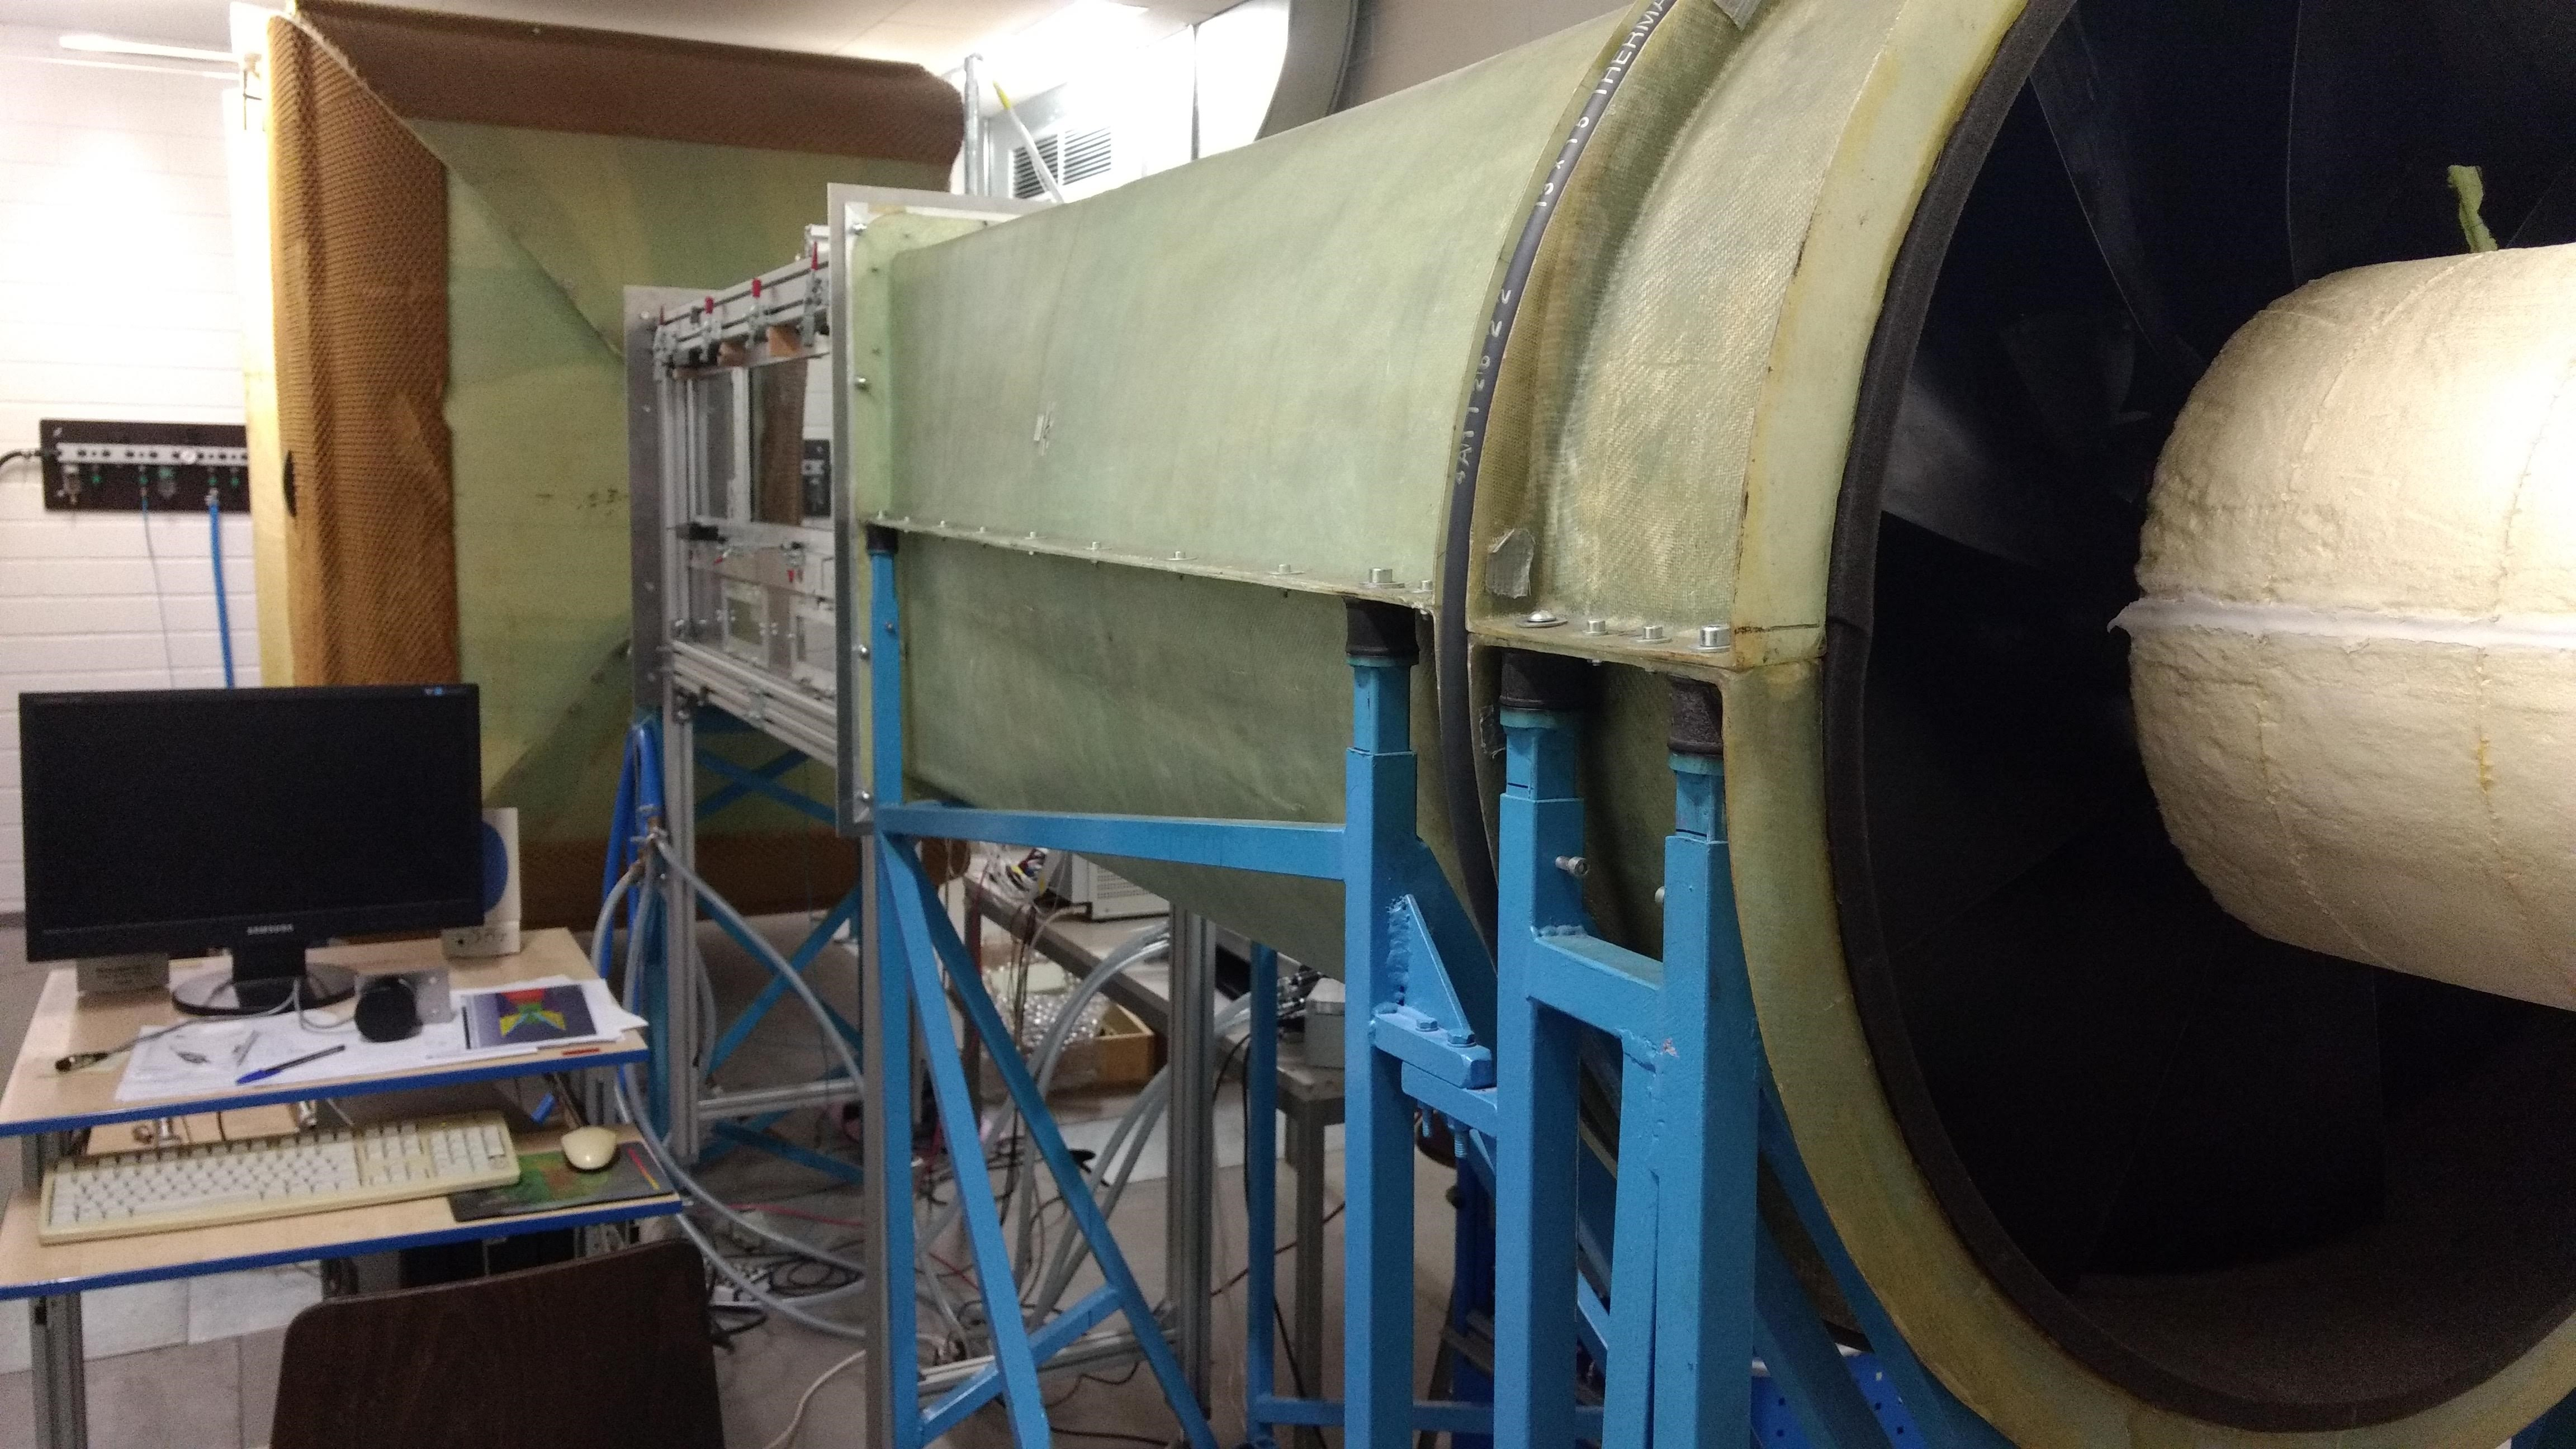
\includegraphics[width=1\textwidth]{windkanal2.jpg}
	\end{subfigure}
	\caption{LNB-ISM TU Braunschweig}
	\label{fig:windkanal}
\end{figure}\\
Testk"orper, die f"ur die Untersuchung eine maximale Anstr"omgeschwindigkeit von \SI{20}{\meter/\second} ben"otigen und die passende Gr"o\ss{}e haben, sind f"ur Versuche in diesem Windkanal geeignet.

\section{Messtechnik (KK)}
Nicht nur bei der Versuchsvorbereitung, sondern auch w"ahrend des Versuchs werden Messger"ate und Einrichtungen ben"otigt, ohne die eine sinnvolle Untersuchung und rechnerische Ermittlungen der Versuchsparameter nicht m"oglich ist.

Hier wird auf die f"ur den Versuch eingesetzten Messmittel und deren Funktionsweisen eingegangen.

\subsection{Messuhr}
Die Messuhr wird f"ur die Messung der L"angendifferenzen oder auch L"angen eingesetzt. Mit einer "ublichen Genauigkeit von \SI{10}{\micro\meter} und einem Messbereich von 5 bis \SI{60}{\milli\meter} eignen sich die Messuhren f"ur Parallelit"ats- und Ebenheitsmessungen.

\subsection{Fischmaul-Sonde}
Die Fischmaul-Sonde ist im Prinzip ein an der Spitze plattgedr"ucktes Pitot-Rohr. Sie eignet sich am besten f"ur Staudruckmessungen an bzw. in angestr"omten Spalten.

\subsection{Statische Sonde}
Die statische Sonde besitzt nur Bohrungen, die tangential zur Str"omung sind und deshalb nur für die Messung des statischen Drucks geeignet sind.
Damit die Bohrungen m"oglichst keinen dynamischen Anteil messen, m"ussen sie sich weit genug entfernt von der Sondenspitze befinden, da in und nach diesem Bereich, die Str"omung umgelenkt wird und lokal nicht mehr tangential zu den Bohrungseintrittsfl"achen steht.

\subsection{Prandtl-Sonde}
Diese Sonde kombiniert die statische Sonde und das Pitot-Rohr.
Die von der seitlichen Bohrungen gemessenen Dr"ucke laufen im inneren System gegen den an der Spitze gemessenen Staudruck.
Somit wird der statische Druck vom Gesamtdruck abgezogen und der dynamische Druck erhalten. Durch weitere Rechnungen ist es m"oglich, mittels dynamischen Drucks die Anstr"omgeschwindigkeiten zu berechnen.

\subsection{Drehzahlmesser}

\subsection{PSI-Anlage}

\section{Versuchsvorbereitung (KK)}
\label{sec:Versuchsvorbereitung}

